% Select document class: uncomment one of the following
\documentclass[aspectratio=169]{beamer}  % For presentation mode
%\documentclass[11pt]{article}            % For article mode
%\usepackage{beamerarticle}               % Uncomment with article class

% =============================================================================
% COMMON PREAMBLE
% =============================================================================
% =============================================================================
% Common Preamble for Network+ Lecture Series
% This file provides consistent formatting, colors, packages, and styles
% across all lecture modules for both beamer presentations and article mode
% =============================================================================

% =============================================================================
% THEME AND COLORS
% =============================================================================
\usetheme{Madrid}
\usecolortheme{whale}

% Custom colors - standardized across all lectures
\definecolor{rctcblue}{RGB}{0, 74, 136}
\definecolor{rctcgold}{RGB}{255, 199, 44}
\definecolor{networkgreen}{RGB}{0, 128, 64}
\definecolor{alertred}{RGB}{180, 0, 0}
\definecolor{aborange}{RGB}{230, 126, 34}
\definecolor{copperbrown}{RGB}{184, 115, 51}
\definecolor{faborange}{RGB}{255, 165, 0}
\definecolor{fiberyellow}{RGB}{255, 215, 0}
\definecolor{shirepurple}{RGB}{102, 51, 153}
\definecolor{ipblue}{RGB}{52, 152, 219}
\definecolor{ippurple}{RGB}{155, 89, 182}
\definecolor{vlangreen}{RGB}{39, 174, 96}
\definecolor{tcpblue}{RGB}{30, 100, 180}
\definecolor{udpgreen}{RGB}{50, 160, 80}
\definecolor{dhcppurple}{RGB}{120, 60, 160}
\definecolor{dnsyellow}{RGB}{200, 170, 50}
\definecolor{batblack}{RGB}{30, 30, 40}
\definecolor{gothamgray}{RGB}{80, 85, 95}
\definecolor{paddysgreen}{RGB}{19, 77, 33}
\definecolor{beerlight}{RGB}{255, 199, 44}
\definecolor{sunnyorange}{RGB}{255, 140, 0}
\definecolor{ogregreen}{RGB}{34, 139, 34}
\definecolor{swampbrown}{RGB}{101, 67, 33}

% Set theme colors
\setbeamercolor{palette primary}{bg=rctcblue,fg=white}
\setbeamercolor{palette secondary}{bg=rctcblue!80,fg=white}
\setbeamercolor{palette tertiary}{bg=rctcblue!60,fg=white}
\setbeamercolor{structure}{fg=rctcblue}
\setbeamercolor{title}{fg=white,bg=rctcblue}
\setbeamercolor{frametitle}{fg=white,bg=rctcblue}
\setbeamercolor{block title}{bg=rctcblue,fg=white}
\setbeamercolor{block body}{bg=rctcblue!10,fg=black}
\setbeamercolor{block title alerted}{bg=alertred,fg=white}
\setbeamercolor{block body alerted}{bg=alertred!10,fg=black}
\setbeamercolor{block title example}{bg=networkgreen,fg=white}
\setbeamercolor{block body example}{bg=networkgreen!10,fg=black}

% =============================================================================
% PACKAGES
% =============================================================================
\usepackage[utf8]{inputenc}
\usepackage[T1]{fontenc}
\usepackage{lmodern}  % Better font rendering
\usepackage{graphicx}
\usepackage{tikz}
\usepackage{booktabs}
\usepackage{array}
\usepackage{multirow}
\usepackage{hyperref}
\usepackage{adjustbox}
\usepackage{amssymb}
\usepackage{amsmath}
\usepackage{calc}
\usepackage{fontawesome5}
% xcolor with [table] option: avoid colortbl.4ht hook conflict in tex4ht
\ifdefined\HCode
  \usepackage{xcolor}
  \usepackage{colortbl}  % provides \rowcolor etc.
\else
  \usepackage[table]{xcolor}  % includes colortbl for pdflatex
\fi

% =============================================================================
% TIKZ LIBRARIES AND SETUP
% =============================================================================
\usetikzlibrary{
    shapes.geometric,
    shapes.symbols,
    shapes.misc,
    arrows.meta,
    positioning,
    calc,
    fit,
    backgrounds,
    decorations.pathreplacing,
    decorations.pathmorphing,
    matrix,
    chains
}
% shadows library causes pgfuseshading errors with tex4ht;
% only load it when NOT building HTML
\ifdefined\HCode\else
    \usetikzlibrary{shadows}
\fi

% Graphics path for icons and chapter images
\graphicspath{
    {../images/icons/}
    {./images/icons/}
    {images/icons/}
    {../images/ch1/}
    {./images/ch1/}
    {images/ch1/}
    {../images/ch2/}
    {./images/ch2/}
    {images/ch2/}
    {../images/ch3/}
    {./images/ch3/}
    {images/ch3/}
    {../images/ch4/}
    {./images/ch4/}
    {images/ch4/}
    {../images/ch5/}
    {./images/ch5/}
    {images/ch5/}
    {../images/ch6/}
    {./images/ch6/}
    {images/ch6/}
    {../images/ch7/}
    {./images/ch7/}
    {images/ch7/}
    {../images/ch8/}
    {./images/ch8/}
    {images/ch8/}
    {../images/ch9/}
    {./images/ch9/}
    {images/ch9/}
    {../images/}
    {./images/}
    {images/}
}

% =============================================================================
% NETWORK DIAGRAM STYLES
% =============================================================================
\tikzset{
    % Node styles for network devices
    device/.style={
        inner sep=2pt,
        label distance=2pt
    },
    pc/.style={device},
    laptop/.style={device},
    server/.style={device},
    router/.style={device},
    switch/.style={device},
    firewall/.style={device},
    cloud/.style={device},
    phone/.style={device},
    tablet/.style={device},
    wifi/.style={device},
    % Connection styles
    ethernet/.style={
        draw=rctcblue,
        line width=1.5pt,
        -{Stealth[length=3mm]}
    },
    ethernet noarrow/.style={
        draw=rctcblue,
        line width=1.5pt
    },
    wireless/.style={
        draw=aborange,
        line width=1.5pt,
        dashed,
        -{Stealth[length=3mm]}
    },
    wireless noarrow/.style={
        draw=aborange,
        line width=1.5pt,
        dashed
    },
    wan/.style={
        draw=alertred,
        line width=2pt,
        -{Stealth[length=3mm]}
    },
    wan noarrow/.style={
        draw=alertred,
        line width=2pt
    },
    copper/.style={
        draw=copperbrown,
        line width=2pt,
        -{Stealth[length=3mm]}
    },
    copper noarrow/.style={
        draw=copperbrown,
        line width=2pt
    },
    fiber/.style={
        draw=fiberyellow,
        line width=2pt,
        -{Stealth[length=3mm]}
    },
    fiber noarrow/.style={
        draw=fiberyellow,
        line width=2pt
    },
    trunk/.style={
        draw=shirepurple,
        line width=2pt,
        -{Stealth[length=3mm]}
    },
    trunk noarrow/.style={
        draw=shirepurple,
        line width=2pt
    },
    % Packet/segment styles
    pktseg/.style={
        draw=rctcblue,
        fill=rctcblue!10,
        minimum height=0.5cm,
        font=\tiny,
        rounded corners=2pt
    },
    pktseg tcp/.style={
        draw=tcpblue,
        fill=tcpblue!15,
        minimum height=0.5cm,
        font=\tiny,
        rounded corners=2pt
    },
    pktseg udp/.style={
        draw=udpgreen,
        fill=udpgreen!15,
        minimum height=0.5cm,
        font=\tiny,
        rounded corners=2pt
    },
    pktseg highlight/.style={
        draw=aborange,
        fill=aborange!20,
        minimum height=0.5cm,
        font=\tiny,
        rounded corners=2pt
    },
    % Box styles
    ipbox/.style={
        draw=rctcblue,
        fill=rctcblue!10,
        rounded corners,
        minimum height=0.4cm,
        font=\small
    },
    portbox/.style={
        draw=tcpblue,
        fill=tcpblue!10,
        rounded corners,
        minimum height=0.4cm,
        font=\small
    },
    dnsbox/.style={
        draw=dnsyellow,
        fill=dnsyellow!15,
        rounded corners,
        minimum height=0.4cm,
        font=\small
    },
    routetable/.style={
        draw=rctcblue,
        fill=rctcblue!10,
        rounded corners,
        minimum height=0.4cm,
        font=\small
    },
    macbox/.style={
        draw=networkgreen,
        fill=networkgreen!10,
        rounded corners,
        minimum height=0.4cm,
        font=\small
    },
    % Frame segment styles (Ethernet frame diagrams)
    frameseg/.style={
        draw=rctcblue,
        fill=rctcblue!10,
        minimum height=0.5cm,
        font=\tiny,
        rounded corners=2pt
    },
    frameseg highlight/.style={
        draw=aborange,
        fill=aborange!20,
        minimum height=0.5cm,
        font=\tiny,
        rounded corners=2pt
    },
    % Process/flow styles
    process/.style={
        draw=rctcblue,
        fill=rctcblue!15,
        rounded corners,
        minimum width=2cm,
        minimum height=0.6cm,
        font=\small,
        align=center
    },
    decision/.style={
        draw=aborange,
        fill=aborange!15,
        diamond,
        aspect=2,
        minimum width=1.5cm,
        font=\small,
        align=center
    },
    % OSI Layer styles
    osilayer/.style={
        draw=rctcblue,
        fill=rctcblue!10,
        minimum width=3cm,
        minimum height=0.45cm,
        font=\small
    },
    osilayer highlight/.style={
        draw=aborange,
        fill=aborange!20,
        line width=1.5pt,
        minimum width=3cm,
        minimum height=0.45cm,
        font=\small\bfseries
    }
}

% =============================================================================
% ICON COMMANDS - Standardized using PNG files and FontAwesome
% =============================================================================
% Network device icons (PNG)
\newcommand{\iconpc}[1][0.6cm]{\resizebox{#1}{!}{
\includegraphics{icon_pc}}}
\newcommand{\iconlaptop}[1][0.6cm]{\resizebox{#1}{!}{
\includegraphics{icon_laptop}}}
\newcommand{\iconserver}[1][0.6cm]{\resizebox{#1}{!}{
\includegraphics{icon_server}}}
\newcommand{\iconrouter}[1][0.6cm]{\resizebox{#1}{!}{
\includegraphics{icon_router}}}
\newcommand{\iconswitch}[1][0.6cm]{\resizebox{#1}{!}{
\includegraphics{icon_switch}}}
\newcommand{\iconfirewall}[1][0.6cm]{\resizebox{#1}{!}{
\includegraphics{icon_firewall}}}
\newcommand{\iconcloud}[1][0.6cm]{\resizebox{#1}{!}{
\includegraphics{icon_cloud}}}
\newcommand{\iconphone}[1][0.6cm]{\resizebox{#1}{!}{
\includegraphics{icon_phone}}}
\newcommand{\icontablet}[1][0.6cm]{\resizebox{#1}{!}{
\includegraphics{icon_tablet}}}
\newcommand{\iconwifi}[1][0.6cm]{\resizebox{#1}{!}{
\includegraphics{icon_wifi}}}
\newcommand{\icondatabase}[1][0.6cm]{\resizebox{#1}{!}{
\includegraphics{icon_db}}}
\newcommand{\iconlock}[1][0.6cm]{\resizebox{#1}{!}{
\includegraphics{icon_lock}}}

% For HTML/tex4ht builds: replace PNG icons with FontAwesome5 glyphs.
% dvisvgm embeds font glyphs as vectors but silently ignores em:graph (PNG)
% specials, so PNG icons would be blank in the output SVGs. FA5 glyphs work.
\ifdefined\HCode
  \renewcommand{\iconpc}[1][0.6cm]{\resizebox{#1}{!}{\faIcon{desktop}}}
  \renewcommand{\iconlaptop}[1][0.6cm]{\resizebox{#1}{!}{\faIcon{laptop}}}
  \renewcommand{\iconserver}[1][0.6cm]{\resizebox{#1}{!}{\faIcon{server}}}
  \renewcommand{\iconrouter}[1][0.6cm]{\resizebox{#1}{!}{\faIcon{route}}}
  \renewcommand{\iconswitch}[1][0.6cm]{\resizebox{#1}{!}{\faIcon{network-wired}}}
  \renewcommand{\iconfirewall}[1][0.6cm]{\resizebox{#1}{!}{\faIcon{shield-alt}}}
  \renewcommand{\iconcloud}[1][0.6cm]{\resizebox{#1}{!}{\faIcon{cloud}}}
  \renewcommand{\iconphone}[1][0.6cm]{\resizebox{#1}{!}{\faIcon{mobile-alt}}}
  \renewcommand{\icontablet}[1][0.6cm]{\resizebox{#1}{!}{\faIcon{tablet-alt}}}
  \renewcommand{\iconwifi}[1][0.6cm]{\resizebox{#1}{!}{\faIcon{wifi}}}
  \renewcommand{\icondatabase}[1][0.6cm]{\resizebox{#1}{!}{\faIcon{database}}}
  \renewcommand{\iconlock}[1][0.6cm]{\resizebox{#1}{!}{\faIcon{lock}}}
\fi

% FontAwesome icons
\newcommand{\iconuser}[1][0.6cm]{\resizebox{#1}{!}{\faIcon{user}}}
\newcommand{\iconglobe}[1][0.6cm]{\resizebox{#1}{!}{\faIcon{globe}}}
\newcommand{\iconclock}[1][0.6cm]{\resizebox{#1}{!}{\faIcon{clock}}}
\newcommand{\iconmail}[1][0.6cm]{\resizebox{#1}{!}{\faIcon{envelope}}}
\newcommand{\icondoc}[1][0.6cm]{\resizebox{#1}{!}{\faIcon{file-alt}}}
\newcommand{\iconsearch}[1][0.6cm]{\resizebox{#1}{!}{\faIcon{search}}}
\newcommand{\icontools}[1][0.6cm]{\resizebox{#1}{!}{\faIcon{tools}}}
\newcommand{\iconchart}[1][0.6cm]{\resizebox{#1}{!}{\faIcon{chart-line}}}
\newcommand{\iconalert}[1][0.6cm]{\resizebox{#1}{!}{\faIcon{bell}}}
\newcommand{\iconlog}[1][0.6cm]{\resizebox{#1}{!}{\faIcon{clipboard-list}}}
\newcommand{\iconeye}[1][0.6cm]{\resizebox{#1}{!}{\faIcon{eye}}}
\newcommand{\iconhacker}[1][0.6cm]{\resizebox{#1}{!}{\faIcon{user-secret}}}
\newcommand{\iconkey}[1][0.6cm]{\resizebox{#1}{!}{\faIcon{key}}}
\newcommand{\iconfile}[1][0.6cm]{\resizebox{#1}{!}{\faIcon{file-alt}}}
\newcommand{\icondog}[1][0.6cm]{\resizebox{#1}{!}{\faIcon{dog}}}
\newcommand{\iconcat}[1][0.6cm]{\resizebox{#1}{!}{\faIcon{cat}}}
\newcommand{\iconvoip}[1][0.6cm]{\resizebox{#1}{!}{\faIcon{phone-volume}}}
\newcommand{\iconmoney}[1][0.6cm]{\resizebox{#1}{!}{\faIcon{money-bill-wave}}}
\newcommand{\icontrash}[1][0.6cm]{\resizebox{#1}{!}{\faIcon{trash}}}
\newcommand{\iconbuilding}[1][0.6cm]{\resizebox{#1}{!}{\faIcon{building}}}

% =============================================================================
% CUSTOM COMMANDS AND ENVIRONMENTS
% =============================================================================

% Key term formatting
\newcommand{\keyterm}[1]{\textbf{#1}}

% Slide section marker
\newcommand{\sectionslide}[1]{
    \begin{frame}
        \vfill
        \centering
        \begin{beamercolorbox}[sep=8pt,center,shadow=true,rounded=true]{title}
            \usebeamerfont{title}\Huge #1
        \end{beamercolorbox}
        \vfill
    \end{frame}
}

% Case study frame environment
\newenvironment{casestudy}[1]{%
    \begin{alertblock}{$\blacktriangleright$ Case Study: #1}
}{%
    \end{alertblock}
}

% Solution frame environment  
\newenvironment{casesolution}[1]{%
    \begin{exampleblock}{$\checkmark$ Solution: #1}
}{%
    \end{exampleblock}
}

% =============================================================================
% FOOTER WITH SLIDE NUMBERS
% =============================================================================
\setbeamertemplate{footline}{
    \leavevmode%
    \hbox{%
        \begin{beamercolorbox}[wd=.333333\paperwidth,ht=2.25ex,dp=1ex,center]{author in head/foot}%
            \usebeamerfont{author in head/foot}\insertshortauthor
        \end{beamercolorbox}%
        \begin{beamercolorbox}[wd=.333333\paperwidth,ht=2.25ex,dp=1ex,center]{title in head/foot}%
            \usebeamerfont{title in head/foot}\insertshorttitle
        \end{beamercolorbox}%
        \begin{beamercolorbox}[wd=.333333\paperwidth,ht=2.25ex,dp=1ex,right]{date in head/foot}%
            \usebeamerfont{date in head/foot}\insertshortdate{}\hspace*{2em}
            \insertframenumber{} / \inserttotalframenumber\hspace*{2ex}
        \end{beamercolorbox}}%
    \vskip0pt%
}

% =============================================================================
% ARTICLE MODE SUPPORT
% =============================================================================
% The following commands help with beamerarticle mode for HTML conversion

% In article mode, add proper section/subsection support and override environments
\mode<article>{
    % Make sure figure captions work properly
    \setbeamertemplate{caption}[numbered]
    \setbeamertemplate{caption label separator}{: }
    
    % Add some spacing for readability
    \setlength{\parskip}{0.5em}
    \setlength{\parindent}{0pt}
    
    % Article mode versions of case study environments
    \renewenvironment{casestudy}[1]{%
        \vspace{0.3cm}\noindent\textbf{Case Study: #1}\newline\begin{itshape}
    }{%
        \end{itshape}\vspace{0.3cm}
    }
    
    \renewenvironment{casesolution}[1]{%
        \vspace{0.3cm}\noindent\textbf{Solution: #1}\newline\begin{itshape}
    }{%
        \end{itshape}\vspace{0.3cm}
    }
}

% Command to mark content that only appears in article mode
\newcommand{\articleonly}[1]{\mode<article>{#1}}

% Command to mark content that only appears in presentation mode
\newcommand{\presentationonly}[1]{\mode<presentation>{#1}}


% =============================================================================
% DOCUMENT INFO
% =============================================================================
\title[Network+ Module 13.0]{WAN, VPNs, and Remote Management}
\subtitle{Intro to Networks -- Module 13.0}
\author[B. Shea]{Brendan Shea, PhD}
\institute[RCTC]{Rochester Community and Technical College\\Intro to Networking}
\date{}

\begin{document}

% =============================================================================
% SLIDE 1: Title
% =============================================================================
\begin{frame}
    \titlepage
    \begin{center}
        \begin{tikzpicture}[scale=0.85]
            % Home user
            \node[laptop] (home) at (0,0) {\iconlaptop[0.5cm]};
            \node[font=\tiny, below=0.05cm of home] {Remote User};
            % Internet cloud
            \node[cloud] (cloud) at (4.5,0) {\iconcloud[0.65cm]};
            \node[font=\tiny, below=0.1cm of cloud] {Internet};
            % Firewall
            \node[firewall] (fw) at (7.5,0) {\iconfirewall[0.5cm]};
            % HQ server
            \node[server] (srv) at (9.5,0) {\iconserver[0.5cm]};
            \node[font=\tiny, below=0.05cm of srv] {HQ Server};
            % Connections
            \draw[ethernet noarrow, line width=1.2pt] (home) -- (1.3,0);
            \draw[alertred, line width=2pt, dashed] (1.3,0) -- (3.2,0);
            \draw[alertred, line width=2pt, dashed] (5.8,0) -- (fw);
            \draw[ethernet noarrow, line width=1.2pt] (fw) -- (srv);
            % Lock icons
            \node[font=\normalsize, networkgreen] at (2.3,0.4) {\faIcon{lock}};
            \node[font=\normalsize, networkgreen] at (6.5,0.4) {\faIcon{lock}};
            \node[font=\tiny\bfseries, aborange] at (4.5,0.6) {VPN Tunnel};
            % Branch below
            \node[router] (br) at (4.5,-1.5) {\iconrouter[0.45cm]};
            \node[font=\tiny, below=0.05cm of br] {Branch Office};
            \node[pc] (brpc) at (2.5,-1.5) {\iconpc[0.35cm]};
            \draw[ethernet noarrow, line width=1pt] (brpc) -- (br);
            \draw[alertred, line width=2pt, dashed] (br) -- (4.5,-0.7);
            \node[font=\tiny\bfseries, aborange] at (6.5,-1.1) {Site-to-Site VPN};
        \end{tikzpicture}
    \end{center}
\end{frame}

% Table of contents in presentation mode only
\presentationonly{
\begin{frame}[allowframebreaks]{Outline}
\small
\tableofcontents[hideallsubsections]
\end{frame}
}

% =============================================================================
% SLIDE 2: Review from Module 12
% =============================================================================
\section*{Review from Module 12}

\begin{frame}{Review: From Wireless LANs to Wide Area Networks}
    \begin{columns}[T]
        \begin{column}{0.55\textwidth}
            \begin{block}{Key Module 12 Concepts}
                \begin{itemize}
                    \item \textbf{802.11 (Wi-Fi)} connects devices on a local wireless network.
                    \item An \textbf{Access Point (AP)} bridges wireless clients to the wired LAN.
                    \item Wi-Fi covers a building or campus --- but \textit{not} the distance between cities.
                \end{itemize}
            \end{block}
            \vspace{0.3em}
            \begin{exampleblock}{The Question for Module 13}
                How do networks in \textit{different cities or countries} communicate securely?
                That requires \textbf{WAN links}, \textbf{VPNs}, and \textbf{remote management} tools.
            \end{exampleblock}
        \end{column}
        \begin{column}{0.42\textwidth}
            \begin{center}
                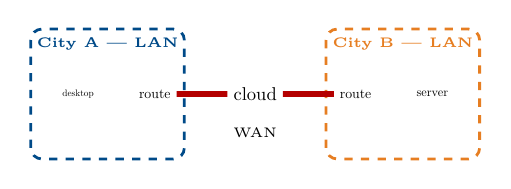
\begin{tikzpicture}[scale=0.75]
                    % City A
                    \draw[dashed, rctcblue, rounded corners, line width=1pt]
                        (-0.8,-0.4) rectangle (1.8,1.8);
                    \node[font=\tiny\bfseries, rctcblue] at (0.5,1.55) {City A --- LAN};
                    \node[pc] at (0,0.7) {\iconpc[0.4cm]};
                    \node[router] (ra) at (1.3,0.7) {\iconrouter[0.4cm]};
                    % WAN cloud
                    \node[cloud] (cloud) at (3,0.7) {\iconcloud[0.55cm]};
                    \node[font=\tiny] at (3,0.05) {WAN};
                    % City B
                    \draw[dashed, aborange, rounded corners, line width=1pt]
                        (4.2,-0.4) rectangle (6.8,1.8);
                    \node[font=\tiny\bfseries, aborange] at (5.5,1.55) {City B --- LAN};
                    \node[router] (rb) at (4.7,0.7) {\iconrouter[0.4cm]};
                    \node[server] at (6.0,0.7) {\iconserver[0.4cm]};
                    % WAN links
                    \draw[wan noarrow] (ra) -- (cloud);
                    \draw[wan noarrow] (cloud) -- (rb);
                \end{tikzpicture}
                \par\tiny\textit{Two LANs connected by a provider-owned WAN --- the topic of this module.}
            \end{center}
        \end{column}
    \end{columns}
\end{frame}

% =============================================================================
% SLIDE 3: Learning Outcomes
% =============================================================================
\begin{frame}[t,allowframebreaks]{Learning Outcomes}
    After completing this module, you will be able to:
    \vspace{0.4em}
    \begin{itemize}
        \item Describe common \keyterm{WAN} technologies and choose the right one for a scenario.
        \item Distinguish between \keyterm{Fiber to the Curb (FTTC)} and \keyterm{Fiber to the Premises (FTTP)}.
        \item Explain what a \keyterm{VPN} is and why it is needed for secure remote communication.
        \item Describe how \keyterm{tunneling} and \keyterm{encapsulation} protect data in transit.
        \item Identify common tunneling protocols: PPTP, L2TP/IPsec, OpenVPN, WireGuard.
        \item Explain \keyterm{IPsec} and the difference between \keyterm{AH} and \keyterm{ESP}, and Transport vs.\ Tunnel mode.
        \item Describe the two phases of \keyterm{IKE} (Internet Key Exchange).
        \item Compare \keyterm{client-to-site}, \keyterm{clientless}, and \keyterm{site-to-site} VPNs.
        \item Use remote management tools: \keyterm{SSH}, \keyterm{Telnet}, \keyterm{RDP}.
        \item Explain \keyterm{out-of-band management}, \keyterm{jump boxes}, and \keyterm{API} access.
    \end{itemize}
\end{frame}

% =============================================================================
% SECTION 1: WAN AND INTERNET CONNECTIVITY
% =============================================================================
\section{WAN and Internet Connectivity}
\subsection{WAN Basics and Access Technologies}

\sectionslide{Section 1: WAN and Internet Connectivity}

% =============================================================================
% SLIDE 5: What Is a WAN?
% =============================================================================
\begin{frame}{What Is a WAN?}
    \begin{columns}[T]
        \begin{column}{0.52\textwidth}
            \begin{itemize}
                \item A \keyterm{Wide Area Network (WAN)} connects networks that are geographically separated --- different buildings, cities, or countries.
                \item Unlike a LAN, you \textbf{do not own} the WAN infrastructure.
                      You \textit{rent} it from an \keyterm{Internet Service Provider (ISP)}.
                \item WANs operate across OSI \textbf{Layers 1--3}: physical media, data link framing, and IP routing at the edges.
            \end{itemize}
            \vspace{0.3em}
            \begin{exampleblock}{Everyday Example}
                When you load a website, your data travels: home LAN $\rightarrow$ ISP's WAN $\rightarrow$ internet $\rightarrow$ a server somewhere else. You own the first hop; the ISP owns the rest.
            \end{exampleblock}
        \end{column}
        \begin{column}{0.45\textwidth}
            \begin{center}
                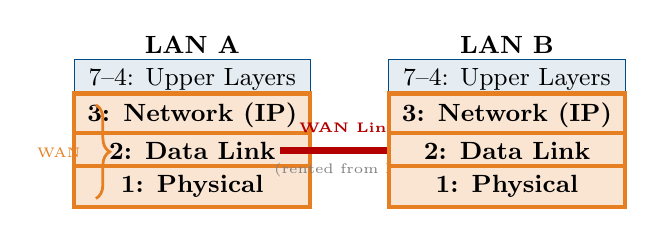
\begin{tikzpicture}[scale=0.72]
                    % LAN A stack
                    \node[osilayer] (a7) at (0,3.15) {7--4: Upper Layers};
                    \node[osilayer highlight] (a3) at (0,2.52) {3: Network (IP)};
                    \node[osilayer highlight] (a2) at (0,1.89) {2: Data Link};
                    \node[osilayer highlight] (a1) at (0,1.26) {1: Physical};
                    \node[font=\small\bfseries] at (0,3.75) {LAN A};
                    % WAN link arrow
                    \draw[wan noarrow, line width=2.5pt] (1.55,1.89) -- (4.0,1.89);
                    \node[font=\tiny\bfseries, alertred] at (2.75,2.3) {WAN Link};
                    \node[font=\tiny, gray] at (2.75,1.55) {(rented from ISP)};
                    % LAN B stack
                    \node[osilayer] at (5.55,3.15) {7--4: Upper Layers};
                    \node[osilayer highlight] at (5.55,2.52) {3: Network (IP)};
                    \node[osilayer highlight] at (5.55,1.89) {2: Data Link};
                    \node[osilayer highlight] at (5.55,1.26) {1: Physical};
                    \node[font=\small\bfseries] at (5.55,3.75) {LAN B};
                    % Brace label
                    \draw[decorate,decoration={brace,amplitude=5pt,mirror},
                          line width=1pt, aborange]
                        (-1.7,1.05) -- (-1.7,2.7);
                    \node[font=\tiny, aborange, left] at (-1.8,1.85) {WAN};
                \end{tikzpicture}
                \par\tiny\textit{WANs operate at Layers 1--3. Upper-layer processing happens at each LAN endpoint.}
            \end{center}
        \end{column}
    \end{columns}
\end{frame}

\articleonly{
\par\small\emph{The diagram shows two OSI stacks (LAN A and LAN B) with Layers 1--3 highlighted in orange. A red WAN Link arrow bridges the two stacks at the Data Link/Network layer boundary, labeled as rented ISP infrastructure. Upper layers (4--7) are local to each site and are not involved in the WAN link itself.}\par
}

% =============================================================================
% SLIDE 6: Internet Access Types Table
% =============================================================================
\begin{frame}[t]{Internet Access Types: Overview}
    \begin{center}
        \footnotesize
        \begin{tabular}{l l l c l}
            \toprule
            \textbf{Technology} & \textbf{Medium} & \textbf{Typical Speed} & \textbf{Shared?} & \textbf{Best For} \\
            \midrule
            \rowcolor{ipblue!15}
            DSL          & Copper phone line & 1--100 Mbps       & No          & Suburban, rural \\
            \rowcolor{networkgreen!15}
            Cable (DOCSIS) & Coaxial cable   & 25 Mbps--1 Gbps   & \textbf{Yes} & Urban, suburban \\
            \rowcolor{rctcblue!10}
            Fiber (FTTP)   & Fiber optic     & 100 Mbps--10 Gbps & No          & Best performance \\
            \rowcolor{aborange!15}
            Fixed Wireless & Radio           & 25--300 Mbps      & Yes         & Rural, backup \\
            \rowcolor{alertred!10}
            Satellite (LEO) & RF (low-orbit) & 25--300 Mbps      & Yes         & Remote locations \\
            \rowcolor{ippurple!10}
            Cellular (4G/5G) & RF            & 10 Mbps--1 Gbps   & Yes         & Mobile, failover \\
            \bottomrule
        \end{tabular}
    \end{center}
    \vspace{0.4em}
    \begin{columns}[T]
        \begin{column}{0.48\textwidth}
            \begin{alertblock}{Shared vs.\ Dedicated}
                \footnotesize
                A \textbf{shared} medium means your neighbors use the same capacity. Speeds drop when the network is busy --- for example, cable internet often slows on weekday evenings.
            \end{alertblock}
        \end{column}
        \begin{column}{0.48\textwidth}
            \begin{block}{Key Vocabulary}
                \footnotesize
                \textbf{Bandwidth}: maximum possible data rate \\
                \textbf{Latency}: delay in milliseconds per packet \\
                \textbf{Throughput}: actual delivered speed
            \end{block}
        \end{column}
    \end{columns}
\end{frame}

% =============================================================================
% SLIDE 7: DSL and Cable
% =============================================================================
\begin{frame}[t]{DSL and Cable Internet}
    \begin{columns}[T]
        \begin{column}{0.48\textwidth}
            \begin{block}{DSL --- Digital Subscriber Line}
                \begin{itemize}
                    \footnotesize
                    \item Uses existing \textbf{telephone copper} wiring to the home.
                    \item \textbf{Dedicated} line per subscriber --- neighbors do not share your speed.
                    \item Speed drops with \textbf{distance} from the ISP's central office.
                    \item \textbf{ADSL}: asymmetric --- faster download than upload.
                    \item \textbf{VDSL}: faster than ADSL but shorter maximum range.
                    \item Customer device: \textbf{DSL modem} (plus router).
                \end{itemize}
            \end{block}
        \end{column}
        \begin{column}{0.48\textwidth}
            \begin{block}{Cable --- DOCSIS}
                \begin{itemize}
                    \footnotesize
                    \item Uses \textbf{coaxial cable} (same physical cable as TV service).
                    \item \textbf{Shared} among homes in a neighborhood node.
                    \item \keyterm{DOCSIS} (Data Over Cable Service Interface Specification) is the industry standard.
                    \item DOCSIS 3.1 supports over \textbf{1 Gbps} downstream.
                    \item Customer device: \textbf{cable modem} (plus router).
                \end{itemize}
            \end{block}
        \end{column}
    \end{columns}
    \vspace{0.3em}
    \begin{center}
        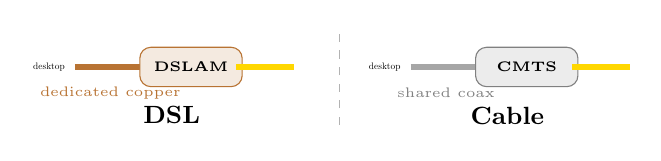
\begin{tikzpicture}[scale=0.82]
            % DSL side
            \node[pc] at (0,0) {\iconpc[0.4cm]};
            \draw[copper noarrow, line width=2pt] (0.4,0) -- (1.5,0);
            \node[draw=copperbrown, fill=copperbrown!15, rounded corners,
                  font=\tiny\bfseries, minimum width=1.3cm, minimum height=0.5cm] at (2.2,0) {DSLAM};
            \draw[fiber noarrow, line width=2pt] (2.9,0) -- (3.8,0);
            \node[font=\tiny, copperbrown] at (0.95,-0.4) {dedicated copper};
            \node[font=\small\bfseries] at (1.9,-0.75) {DSL};
            % Divider
            \draw[gray!60, dashed] (4.5,-0.9) -- (4.5,0.6);
            % Cable side
            \node[pc] at (5.2,0) {\iconpc[0.4cm]};
            \draw[draw=gray!70, line width=2.5pt] (5.6,0) -- (6.7,0);
            \node[draw=gray, fill=gray!15, rounded corners,
                  font=\tiny\bfseries, minimum width=1.3cm, minimum height=0.5cm] at (7.4,0) {CMTS};
            \draw[fiber noarrow, line width=2pt] (8.1,0) -- (9.0,0);
            \node[font=\tiny, gray] at (6.15,-0.4) {shared coax};
            \node[font=\small\bfseries] at (7.1,-0.75) {Cable};
        \end{tikzpicture}
        \par\tiny\textit{DSL uses dedicated copper to a DSLAM at the central office; cable uses shared coaxial cable to a CMTS. Both backhaul to the ISP via fiber.}
    \end{center}
\end{frame}

\articleonly{
\par\small\emph{The diagram compares DSL and cable last-mile connections. On the DSL side, a PC connects via dedicated copper to a DSLAM (Digital Subscriber Line Access Multiplexer), which feeds into a fiber backhaul. On the cable side, a PC connects via shared coaxial cable to a CMTS (Cable Modem Termination System), which also feeds into fiber. The key distinction is that DSL copper is dedicated per customer while coax is shared among neighbors.}\par
}

% =============================================================================
% SLIDE 8: FTTC vs FTTP
% =============================================================================
\begin{frame}[t,shrink=5]{Fiber to the Curb vs.\ Fiber to the Premises}
    \begin{columns}[T]
        \begin{column}{0.48\textwidth}
            \begin{block}{FTTC --- Fiber to the Curb / Node}
                \begin{itemize}
                    \footnotesize
                    \item \textbf{Fiber} runs from the ISP to a street cabinet near your home.
                    \item The final 100--300 meters use \textbf{copper} (phone line or coax).
                    \item Less expensive to deploy --- no fiber trench to every door.
                    \item Speed is \textbf{limited by the copper tail}; the longer the copper, the slower the speed.
                    \item Many ISPs advertise this as ``fiber'' --- it is not pure fiber.
                \end{itemize}
            \end{block}
        \end{column}
        \begin{column}{0.48\textwidth}
            \begin{block}{FTTP / FTTH --- Fiber to the Premises / Home}
                \begin{itemize}
                    \footnotesize
                    \item \textbf{Pure fiber} from the ISP all the way to your home.
                    \item An \keyterm{ONT (Optical Network Terminal)} at the home converts light signals to Ethernet.
                    \item Best possible speeds and lowest latency --- no copper bottleneck.
                    \item Higher deployment cost due to trenching fiber to every building.
                    \item Example services: Google Fiber, many municipal broadband networks.
                \end{itemize}
            \end{block}
        \end{column}
    \end{columns}
    \vspace{0.3em}
    \begin{center}
        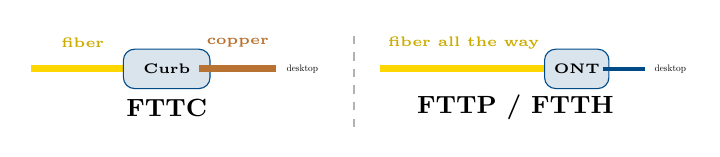
\begin{tikzpicture}[scale=0.82]
            % FTTC
            \draw[fiber noarrow, line width=2.5pt] (0,0.6) -- (1.6,0.6);
            \node[draw=rctcblue, fill=rctcblue!15, rounded corners,
                  font=\tiny\bfseries, minimum width=1.1cm, minimum height=0.5cm] at (2.1,0.6) {Curb};
            \draw[copper noarrow, line width=2.5pt] (2.6,0.6) -- (3.8,0.6);
            \node[pc] at (4.2,0.6) {\iconpc[0.4cm]};
            \node[font=\tiny\bfseries, fiberyellow!80!black] at (0.8,1.0) {fiber};
            \node[font=\tiny\bfseries, copperbrown] at (3.2,1.0) {copper};
            \node[font=\small\bfseries] at (2.1,0.0) {FTTC};
            % Divider
            \draw[gray!60, dashed] (5.0,-0.3) -- (5.0,1.2);
            % FTTP
            \draw[fiber noarrow, line width=2.5pt] (5.4,0.6) -- (8.0,0.6);
            \node[draw=rctcblue, fill=rctcblue!15, rounded corners,
                  font=\tiny\bfseries, minimum width=0.8cm, minimum height=0.5cm] at (8.45,0.6) {ONT};
            \draw[ethernet noarrow, line width=1.5pt] (8.85,0.6) -- (9.5,0.6);
            \node[pc] at (9.9,0.6) {\iconpc[0.4cm]};
            \node[font=\tiny\bfseries, fiberyellow!80!black] at (6.7,1.0) {fiber all the way};
            \node[font=\small\bfseries] at (7.5,0.0) {FTTP / FTTH};
        \end{tikzpicture}
        \par\tiny\textit{FTTC stops fiber at a street cabinet and uses copper for the final run. FTTP runs fiber directly to an ONT at the home.}
    \end{center}
    \begin{alertblock}{\footnotesize Ask Your ISP!}
        \footnotesize When an ISP advertises ``fiber internet,'' always ask: is fiber going all the way to \textit{your door} (FTTP), or only to the street cabinet (FTTC)?
    \end{alertblock}
\end{frame}

\articleonly{
\par\small\emph{The diagram shows two side-by-side last-mile scenarios. FTTC: fiber (yellow arrow) reaches a curb-side cabinet, then copper (brown arrow) completes the run to a home PC. FTTP: fiber continues all the way to an ONT device at the home, after which a short Ethernet cable reaches the PC. The copper segment in FTTC is the speed bottleneck that FTTP eliminates.}\par
}

% =============================================================================
% SLIDE 9: Wireless WAN
% =============================================================================
\begin{frame}[t]{Wireless WAN: Cellular and Satellite}
    \begin{columns}[T]
        \begin{column}{0.50\textwidth}
            \begin{block}{Cellular WAN (4G LTE / 5G)}
                \begin{itemize}
                    \footnotesize
                    \item A \keyterm{cellular router} with a SIM card provides broadband over the mobile network.
                    \item Common uses: primary WAN at remote sites, \textbf{failover backup} if wired WAN fails, IoT devices in the field.
                    \item \textbf{5G sub-6 GHz}: broad coverage, 100--500 Mbps typical.
                    \item \textbf{5G mmWave}: very fast but extremely short range --- dense urban areas only.
                    \item Bandwidth is \textbf{shared} with all mobile users on the tower.
                \end{itemize}
            \end{block}
        \end{column}
        \begin{column}{0.47\textwidth}
            \begin{block}{Satellite Internet}
                \begin{itemize}
                    \footnotesize
                    \item \keyterm{GEO (Geostationary)}: satellite at 35,786 km. \textbf{High latency} $\approx$600 ms RTT --- poor for voice/video.
                    \item \keyterm{LEO (Low-Earth Orbit)}: constellations at $\sim$500 km. \textbf{Low latency} $\approx$20--40 ms. Example: Starlink.
                    \item Best for: locations with no wired or cellular option.
                    \item Both are weather-sensitive and have shared capacity.
                \end{itemize}
            \end{block}
        \end{column}
    \end{columns}
    \vspace{0.3em}
    \begin{exampleblock}{Real-World Use: Automatic Failover}
        \footnotesize
        Many businesses use cellular WAN as a \textbf{secondary / backup} link. If the primary fiber circuit fails, the router automatically switches to LTE --- keeping operations online within seconds. This is called \textbf{WAN failover}.
    \end{exampleblock}
\end{frame}

% =============================================================================
% SLIDE 10: Case Study 1
% =============================================================================
\begin{frame}[t]{Case Study: Tails Sets Up the Freedom Fighter Network}
    \begin{casestudy}{Tails Sets Up the Freedom Fighter Network}
        \footnotesize
        Miles ``Tails'' Prower is building internet connectivity for three Freedom Fighter outposts on Mobius.
        Each needs at least \textbf{50 Mbps} for video surveillance and team coordination.

        \vspace{0.3em}
        \begin{center}
            \begin{tabular}{l p{8cm}}
                \toprule
                \textbf{Outpost}              & \textbf{Situation} \\
                \midrule
                Alpha --- Central City        & A fiber ISP has service available at the building. \\
                Beta --- Mystic Ruins         & No fiber or cable; a 5G tower is visible 2 km away. \\
                Gamma --- Space Colony ARK    & Only satellite service can reach this location. \\
                \bottomrule
            \end{tabular}
        \end{center}

        \vspace{0.3em}
        Tails also notices: Outpost Gamma's video calls have a \textbf{1.2-second audio delay}, and
        Beta's cellular link drops to \textbf{30 Mbps} during peak evening hours.
    \end{casestudy}

    \begin{block}{Review Questions}
        \begin{enumerate}
            \footnotesize
            \item Which WAN technology should each outpost use, and why?
            \item What causes Beta's speed to drop, and what is one solution?
            \item What causes Gamma's 1.2-second audio delay?
        \end{enumerate}
    \end{block}
\end{frame}

% =============================================================================
% SLIDE 11: Case Study 1 Solution
% =============================================================================
\begin{frame}[t]{Case Study Solution: Tails' Freedom Fighter Network}
    \begin{casesolution}{Tails' Freedom Fighter Network}
        \begin{enumerate}
            \footnotesize
            \item \textbf{Alpha $\rightarrow$ FTTP fiber}: Available and provides the best speed and lowest latency. \\
                  \textbf{Beta $\rightarrow$ Cellular WAN (5G)}: No wired option; the nearby 5G tower can meet 50 Mbps with good signal. Use a cellular router with a directional antenna pointed at the tower. \\
                  \textbf{Gamma $\rightarrow$ LEO satellite}: Only satellite reaches the ARK. Use LEO (e.g., Starlink), \textit{not} GEO, to keep latency manageable.
            \item \textbf{Cause}: Cellular is a \textit{shared} medium; tower congestion during peak hours reduces throughput.\\
                  \textbf{Solution}: Add a second cellular modem on a different carrier (carrier diversity) or use \textbf{WAN bonding} to combine two cellular links.
            \item \textbf{GEO satellite latency.} GEO satellites orbit at 35,786 km; the round-trip signal propagation alone is $\sim$600 ms, producing a 1.2-second conversation delay. Switching to LEO ($\approx$40 ms RTT) would largely eliminate the problem.
        \end{enumerate}
    \end{casesolution}
    \vspace{0.2em}
    \begin{alertblock}{Key Lesson}
        \footnotesize Match the WAN technology to site constraints: availability, speed requirement, latency tolerance, and budget. There is rarely one correct answer for all sites.
    \end{alertblock}
\end{frame}

% =============================================================================
% SECTION 2: VIRTUAL PRIVATE NETWORKS
% =============================================================================
\section{Virtual Private Networks}
\subsection{VPN Concepts, Tunneling, and IPsec}

\sectionslide{Section 2: Virtual Private Networks (VPNs)}

% =============================================================================
% SLIDE 13: What Is a VPN?
% =============================================================================
\begin{frame}[t]{What Is a VPN?}
    \begin{columns}[T]
        \begin{column}{0.50\textwidth}
            \begin{itemize}
                \item The public internet is \textbf{not private} --- packets can be intercepted by anyone on the path.
                \item A \keyterm{VPN (Virtual Private Network)} creates a secure, private channel \textit{through} the public internet.
                \item Every VPN needs three things:
                    \begin{enumerate}
                        \footnotesize
                        \item \textbf{Tunneling} --- wraps your packet inside another packet.
                        \item \textbf{Encryption} --- scrambles data so only the endpoints can read it.
                        \item \textbf{Authentication} --- proves each side is who they claim to be.
                    \end{enumerate}
            \end{itemize}
            \vspace{0.3em}
            \begin{exampleblock}{Analogy}
                \footnotesize A VPN is like putting your letter in a \textbf{locked box} before handing it to the postal service. Workers carry it --- but cannot read what is inside.
            \end{exampleblock}
        \end{column}
        \begin{column}{0.47\textwidth}
            \begin{center}
                \begin{tikzpicture}[scale=0.82]
                    % Without VPN
                    \node[font=\small\bfseries, alertred] at (2.2,4.0) {Without VPN};
                    \node[laptop] (l1) at (0,3.2) {\iconlaptop[0.4cm]};
                    \node[cloud]  (c1) at (2.2,3.2) {\iconcloud[0.45cm]};
                    \node[server] (s1) at (4.4,3.2) {\iconserver[0.4cm]};
                    \draw[ethernet noarrow, draw=alertred, line width=1.5pt] (l1) -- (c1);
                    \draw[ethernet noarrow, draw=alertred, line width=1.5pt] (c1) -- (s1);
                    \node[font=\tiny, alertred] at (1.1,3.55) {plaintext!};
                    \node[font=\tiny, alertred] at (3.3,3.55) {plaintext!};
                    \node[font=\large, alertred] at (2.2,2.65) {\faIcon{eye}};
                    \node[font=\tiny, alertred] at (2.2,2.3) {(sniffed!)};
                    % Divider
                    \draw[gray, dashed] (-0.5,1.9) -- (4.9,1.9);
                    % With VPN
                    \node[font=\small\bfseries, networkgreen] at (2.2,1.6) {With VPN};
                    \node[laptop] (l2) at (0,0.8) {\iconlaptop[0.4cm]};
                    \node[cloud]  (c2) at (2.2,0.8) {\iconcloud[0.45cm]};
                    \node[server] (s2) at (4.4,0.8) {\iconserver[0.4cm]};
                    \draw[alertred, dashed, line width=2pt] (l2) -- (c2);
                    \draw[alertred, dashed, line width=2pt] (c2) -- (s2);
                    \node[font=\tiny, networkgreen] at (1.1,1.15) {\faIcon{lock} encrypted};
                    \node[font=\tiny, networkgreen] at (3.3,1.15) {\faIcon{lock} encrypted};
                \end{tikzpicture}
                \par\tiny\textit{Without a VPN, traffic on the internet is readable. A VPN encrypts the data so that only the two endpoints can understand it.}
            \end{center}
        \end{column}
    \end{columns}
\end{frame}

\articleonly{
\par\small\emph{Two scenarios are shown. Top (Without VPN): a laptop sends data through an internet cloud to a server over plain red connections; an eye icon below the cloud represents an attacker sniffing plaintext packets. Bottom (With VPN): the same topology uses dashed red (encrypted tunnel) connections; lock icons and "encrypted" labels show the data is protected.}\par
}

% =============================================================================
% SLIDE 14: Tunneling and Common Protocols
% =============================================================================
\begin{frame}[t]{Tunneling and Common VPN Protocols}
    \begin{columns}[T]
        \begin{column}{0.45\textwidth}
            \begin{block}{How Tunneling Works}
                \begin{itemize}
                    \footnotesize
                    \item \keyterm{Encapsulation}: the original private packet is wrapped inside a \textit{new}, publicly-addressed outer packet.
                    \item The outer packet travels across the internet normally.
                    \item At the far \keyterm{tunnel endpoint}, the outer wrapper is removed and the original packet is delivered.
                    \item Think of it as a \textbf{``packet within a packet.''}
                \end{itemize}
            \end{block}
            \vspace{0.2em}
            \begin{alertblock}{\footnotesize Tunneling $\neq$ Security}
                \footnotesize Tunneling alone only \textit{wraps} the packet. You still need \textbf{encryption} to keep the contents private!
            \end{alertblock}
        \end{column}
        \begin{column}{0.52\textwidth}
            \begin{center}
                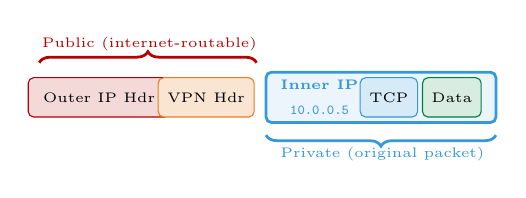
\begin{tikzpicture}[scale=0.8]
                    % Outer IP header
                    \node[pktseg, minimum width=1.8cm, fill=alertred!15, draw=alertred,
                          font=\tiny] (oih) at (0.6,1.8) {Outer IP Hdr};
                    % VPN header
                    \node[pktseg, minimum width=1.2cm, fill=aborange!20, draw=aborange,
                          font=\tiny] (vh) at (2.3,1.8) {VPN Hdr};
                    % Inner packet box
                    \draw[fill=ipblue!10, draw=ipblue, rounded corners=2pt, line width=1pt]
                        (3.25,1.4) rectangle (6.9,2.2);
                    \node[font=\tiny\bfseries, ipblue] at (4.1,2.0) {Inner IP};
                    \node[font=\tiny\ttfamily, ipblue] at (4.1,1.6) {10.0.0.5};
                    \node[pktseg, minimum width=0.7cm, font=\tiny,
                          fill=ipblue!20, draw=ipblue] at (5.2,1.8) {TCP};
                    \node[pktseg, minimum width=0.7cm, font=\tiny,
                          fill=networkgreen!15, draw=networkgreen] at (6.2,1.8) {Data};
                    % Top brace - public
                    \draw[decorate,decoration={brace,amplitude=4pt},
                          line width=1pt, alertred] (-0.35,2.35) -- (3.1,2.35);
                    \node[font=\tiny, alertred] at (1.4,2.65) {Public (internet-routable)};
                    % Bottom brace - private
                    \draw[decorate,decoration={brace,amplitude=4pt,mirror},
                          line width=1pt, ipblue] (3.25,1.2) -- (6.9,1.2);
                    \node[font=\tiny, ipblue] at (5.1,0.9) {Private (original packet)};
                \end{tikzpicture}
                \par\tiny\textit{Encapsulation: the private inner packet is wrapped inside a public outer packet for transit across the internet.}
            \end{center}
            \vspace{0.2em}
            \begin{center}
                \footnotesize
                \begin{tabular}{l l l}
                    \toprule
                    \textbf{Protocol} & \textbf{Encrypted?} & \textbf{Status} \\
                    \midrule
                    PPTP         & Weak (broken) & \textcolor{alertred}{Avoid} \\
                    L2TP/IPsec   & Yes           & Common \\
                    OpenVPN      & Yes (TLS)     & Widely used \\
                    WireGuard    & Yes           & Modern, fast \\
                    SSTP         & Yes (TLS/443) & Windows \\
                    \bottomrule
                \end{tabular}
            \end{center}
        \end{column}
    \end{columns}
\end{frame}

\articleonly{
\par\small\emph{The packet diagram shows three sections: an "Outer IP Hdr" (red) and "VPN Hdr" (orange) that are publicly routable, followed by a blue box containing the private inner IP header, TCP header, and data payload. A red brace labels the outer portion "Public (internet-routable)" and a blue brace labels the inner portion "Private (original packet)." The tunneling protocol table below lists PPTP (broken, avoid), L2TP/IPsec, OpenVPN, WireGuard, and SSTP.}\par
}

% =============================================================================
% SLIDE 15: IPsec
% =============================================================================
\begin{frame}[t]{IPsec: Security Built Into Layer 3}
    \begin{columns}[T]
        \begin{column}{0.48\textwidth}
            \begin{itemize}
                \item \keyterm{IPsec} (Internet Protocol Security) is a \textit{suite} of protocols that adds security directly to IP at Layer 3.
                \item \textbf{Two operating modes:}
                    \begin{itemize}
                        \footnotesize
                        \item \keyterm{Transport mode}: encrypts only the payload; the original IP header stays visible. Used for host-to-host communication.
                        \item \keyterm{Tunnel mode}: encrypts the \textit{entire} original packet and adds a new outer IP header. Used in VPN gateways.
                    \end{itemize}
                \item \textbf{Two sub-protocols:}
                    \begin{itemize}
                        \footnotesize
                        \item \keyterm{AH (Authentication Header)}: provides integrity and authentication --- \textbf{no encryption}.
                        \item \keyterm{ESP (Encapsulating Security Payload)}: provides integrity, authentication, \textit{and} \textbf{encryption}. This is what VPNs use.
                    \end{itemize}
            \end{itemize}
        \end{column}
        \begin{column}{0.49\textwidth}
            \begin{center}
                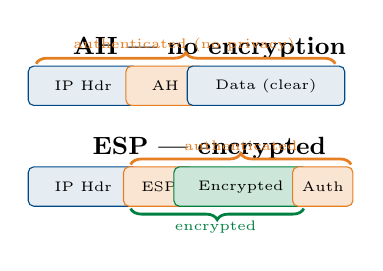
\begin{tikzpicture}[scale=0.8]
                    % AH row
                    \node[font=\small\bfseries] at (2.5,4.1) {AH --- no encryption};
                    \node[pktseg, minimum width=1.4cm] at (0.5,3.5) {IP Hdr};
                    \node[pktseg highlight, minimum width=1.0cm] at (1.8,3.5) {AH};
                    \node[pktseg, minimum width=2.0cm] at (3.4,3.5) {Data (clear)};
                    % Auth bracket over full AH packet
                    \draw[decorate,decoration={brace,amplitude=4pt},
                          line width=1pt, aborange]
                        (-0.25,3.85) -- (4.5,3.85);
                    \node[font=\tiny, aborange] at (2.1,4.15) {authenticated (no privacy)};

                    % ESP row
                    \node[font=\small\bfseries] at (2.5,2.5) {ESP --- encrypted};
                    \node[pktseg, minimum width=1.4cm] at (0.5,1.9) {IP Hdr};
                    \node[pktseg highlight, minimum width=0.9cm] at (1.7,1.9) {ESP};
                    \node[pktseg, minimum width=1.7cm, fill=networkgreen!20,
                          draw=networkgreen] at (3.0,1.9) {Encrypted};
                    \node[pktseg, minimum width=0.7cm, fill=aborange!20,
                          draw=aborange] at (4.3,1.9) {Auth};
                    % Encrypt brace
                    \draw[decorate,decoration={brace,amplitude=4pt,mirror},
                          line width=1pt, networkgreen]
                        (1.25,1.55) -- (4.0,1.55);
                    \node[font=\tiny, networkgreen] at (2.6,1.25) {encrypted};
                    % Auth brace
                    \draw[decorate,decoration={brace,amplitude=4pt},
                          line width=1pt, aborange]
                        (1.25,2.25) -- (4.75,2.25);
                    \node[font=\tiny, aborange] at (3.0,2.55) {authenticated};
                \end{tikzpicture}
                \par\tiny\textit{AH authenticates the entire packet but does not encrypt. ESP both authenticates and encrypts --- always use ESP when privacy is required.}
            \end{center}
            \begin{alertblock}{\footnotesize Use ESP, Not AH Alone}
                \footnotesize AH provides \textit{no confidentiality}. For any VPN carrying private data, always use \textbf{ESP}.
            \end{alertblock}
        \end{column}
    \end{columns}
\end{frame}

\articleonly{
\par\small\emph{Two packet format diagrams are shown. AH packet: IP header, AH header, and Data (cleartext) with an orange brace labeled "authenticated (no privacy)" spanning all fields. ESP packet: IP header, ESP header, Encrypted payload (green), and Auth trailer, with a green brace labeled "encrypted" covering the payload and an orange brace labeled "authenticated" covering ESP through Auth. The diagrams illustrate that AH provides integrity without privacy, while ESP adds encryption.}\par
}

% =============================================================================
% SLIDE 16: IKE
% =============================================================================
\begin{frame}[t]{Internet Key Exchange (IKE)}
    \begin{columns}[T]
        \begin{column}{0.48\textwidth}
            \begin{itemize}
                \item Before IPsec can protect data, both endpoints must agree on \textit{how} --- which algorithms, which keys.
                \item \keyterm{IKE (Internet Key Exchange)} is the protocol that negotiates this agreement automatically.
                \item The agreed-upon parameters are stored in a \keyterm{Security Association (SA)}.
            \end{itemize}
            \vspace{0.3em}
            \begin{block}{Phase 1 --- Authenticate}
                \footnotesize
                Endpoints prove their identities using a \textbf{pre-shared key (PSK)} or a \textbf{digital certificate}. They establish a \textbf{secure, encrypted channel} to negotiate inside.
            \end{block}
            \vspace{0.2em}
            \begin{block}{Phase 2 --- Negotiate Session Keys}
                \footnotesize
                Inside the Phase 1 channel, endpoints agree on the specific \textbf{encryption and hashing algorithms} and generate the \textbf{session keys} that will protect the actual data. This creates the IPsec SA.
            \end{block}
            \vspace{0.2em}
            \begin{exampleblock}{\footnotesize Analogy}
                \footnotesize Phase 1 = showing your ID at the security desk. Phase 2 = agreeing on a secret code before talking business.
            \end{exampleblock}
        \end{column}
        \begin{column}{0.49\textwidth}
            \begin{center}
                \begin{tikzpicture}[scale=0.85]
                    % Routers
                    \node[router] (r1) at (0,4.5) {\iconrouter[0.5cm]};
                    \node[font=\small] at (0,5.1) {Router A};
                    \node[router] (r2) at (5.5,4.5) {\iconrouter[0.5cm]};
                    \node[font=\small] at (5.5,5.1) {Router B};
                    % Phase 1 arrows
                    \draw[-{Stealth}, rctcblue, line width=1.5pt] (0.4,4.2) -- (5.1,3.6);
                    \draw[-{Stealth}, rctcblue, line width=1.5pt] (5.1,3.35) -- (0.4,2.8);
                    \node[font=\tiny\bfseries, rctcblue, fill=white] at (2.75,4.0)
                        {Phase 1: Identity + capabilities};
                    \node[font=\tiny, rctcblue, fill=white] at (2.75,3.2)
                        {PSK or certificate reply};
                    % Phase 1 result
                    \draw[fill=rctcblue!10, draw=rctcblue, rounded corners]
                        (0.6,2.35) rectangle (4.9,2.7);
                    \node[font=\tiny\bfseries] at (2.75,2.52)
                        {Secure Phase 1 channel established};
                    % Phase 2 arrows
                    \draw[-{Stealth}, networkgreen, line width=1.5pt] (0.4,2.0) -- (5.1,1.6);
                    \draw[-{Stealth}, networkgreen, line width=1.5pt] (5.1,1.35) -- (0.4,0.9);
                    \node[font=\tiny\bfseries, networkgreen, fill=white] at (2.75,1.9)
                        {Phase 2: Propose session algorithms};
                    \node[font=\tiny, networkgreen, fill=white] at (2.75,1.2)
                        {Session keys agreed (inside Phase 1)};
                    % Data arrow
                    \draw[-{Stealth}, alertred, dashed, line width=2.5pt] (0.4,0.5) -- (5.1,0.5);
                    \node[font=\tiny\bfseries, alertred] at (2.75,0.8)
                        {\faIcon{lock} \ Encrypted data now flows};
                \end{tikzpicture}
                \par\tiny\textit{IKE Phase 1 authenticates peers and builds a secure channel. Phase 2 negotiates session keys inside that channel. Encrypted data flow begins after Phase 2.}
            \end{center}
        \end{column}
    \end{columns}
\end{frame}

\articleonly{
\par\small\emph{A two-router flow diagram shows IKE phases. Phase 1: bidirectional blue arrows carry "Identity + capabilities" and "PSK or certificate reply" between Router A and Router B, ending with a blue box labeled "Secure Phase 1 channel established." Phase 2: bidirectional green arrows carry session algorithm proposals and key agreement inside the Phase 1 tunnel. Finally, a dashed red arrow labeled "Encrypted data now flows" shows IPsec-protected traffic.}\par
}

% =============================================================================
% SLIDE 17: Client-to-Site VPNs
% =============================================================================
\begin{frame}[t]{Client-to-Site VPNs}
    \begin{columns}[T]
        \begin{column}{0.48\textwidth}
            \begin{itemize}
                \item Also called a \keyterm{remote access VPN}.
                \item An individual user installs \textbf{VPN client software} on their device and connects to a corporate VPN gateway over the internet.
                \item The user is assigned a \textbf{virtual IP address} on the corporate subnet --- their device appears to be physically inside the office.
                \item Common use: employees working from home.
            \end{itemize}
            \vspace{0.3em}
            \begin{block}{Full Tunnel vs.\ Split Tunnel}
                \begin{itemize}
                    \footnotesize
                    \item \keyterm{Full tunnel}: \textit{all} user traffic is routed through the VPN. Most secure; uses more corporate bandwidth.
                    \item \keyterm{Split tunnel}: only corporate-destined traffic uses the VPN; regular internet browsing goes direct. More efficient; slight security trade-off.
                \end{itemize}
            \end{block}
        \end{column}
        \begin{column}{0.49\textwidth}
            \begin{center}
                \begin{tikzpicture}[scale=0.80]
                    % Home laptop
                    \node[laptop] (home) at (0,2.8) {\iconlaptop[0.5cm]};
                    \node[font=\tiny, below=0.05cm of home] {Home Laptop};
                    \node[font=\tiny\ttfamily, ipblue] at (0,2.05) {10.8.0.2 (virtual)};
                    % Internet
                    \node[cloud] (cloud) at (3.2,2.8) {\iconcloud[0.55cm]};
                    \node[font=\tiny] at (3.2,2.15) {Internet};
                    % VPN gateway
                    \node[firewall] (gw) at (6.2,2.8) {\iconfirewall[0.5cm]};
                    \node[font=\tiny, below=0.05cm of gw] {VPN Gateway};
                    % Corporate LAN
                    \draw[dashed, rctcblue, rounded corners, line width=1pt]
                        (7.3,2.1) rectangle (9.3,3.5);
                    \node[server] at (8.3,2.8) {\iconserver[0.4cm]};
                    \node[font=\tiny, rctcblue] at (8.3,3.3) {Corp LAN};
                    \draw[ethernet noarrow, line width=1pt] (gw) -- (7.3,2.8);
                    % Tunnel
                    \draw[alertred, dashed, line width=2pt] (home) -- (cloud);
                    \draw[alertred, dashed, line width=2pt] (cloud) -- (gw);
                    \node[font=\tiny, aborange] at (1.6,3.15) {\faIcon{lock} encrypted};
                    \node[font=\tiny, aborange] at (4.7,3.15) {\faIcon{lock} encrypted};
                    % Split tunnel annotation
                    \draw[-{Stealth}, networkgreen, line width=1pt, dashed]
                        (0.3,2.0) to[bend right=20] (1.8,0.8);
                    \node[font=\tiny, networkgreen, align=center] at (1.5,0.5)
                        {Internet traffic\\(split tunnel: direct)};
                \end{tikzpicture}
                \par\tiny\textit{Client-to-site VPN: the user's VPN software creates an encrypted tunnel to the corporate gateway. With split tunnel, internet-bound traffic bypasses the VPN.}
            \end{center}
        \end{column}
    \end{columns}
\end{frame}

\articleonly{
\par\small\emph{A home laptop (labeled with virtual IP 10.8.0.2) connects via an encrypted dashed tunnel through an internet cloud to a VPN Gateway firewall, beyond which sits the Corporate LAN. Lock icons on the tunnel indicate encryption. A dashed green arrow from the laptop downward-right is labeled "Internet traffic (split tunnel: direct)," showing that with split tunneling, general web browsing exits the internet directly rather than through the VPN.}\par
}

% =============================================================================
% SLIDE 18: Clientless VPNs
% =============================================================================
\begin{frame}[t]{Clientless VPNs (SSL VPN)}
    \begin{columns}[T]
        \begin{column}{0.50\textwidth}
            \begin{itemize}
                \item A \keyterm{clientless VPN} (also called an \keyterm{SSL VPN}) requires \textbf{no software installation} on the user's device.
                \item The user opens a \textbf{web browser}, navigates to a secure portal (HTTPS), and logs in.
                \item The VPN gateway \textbf{proxies} the connection --- fetching internal resources on the user's behalf.
                \item Best for:
                    \begin{itemize}
                        \footnotesize
                        \item Contractors or guests on unmanaged devices.
                        \item Temporary or one-time access to a single web application.
                        \item Environments where software installation is restricted.
                    \end{itemize}
            \end{itemize}
            \vspace{0.2em}
            \begin{alertblock}{Limitation}
                \footnotesize Works only for \textbf{web-based resources} (HTTP/HTTPS). Cannot tunnel arbitrary protocols (file shares, RDP) without a browser plug-in.
            \end{alertblock}
        \end{column}
        \begin{column}{0.47\textwidth}
            \begin{center}
                \begin{tikzpicture}[scale=0.85]
                    % User browser
                    \node[laptop] (lap) at (0,3.2) {\iconlaptop[0.5cm]};
                    \node[font=\tiny, below=0.05cm of lap] {Any Browser};
                    % HTTPS arrow
                    \draw[-{Stealth}, networkgreen, line width=2pt] (0.45,3.2) -- (2.5,3.2);
                    \node[font=\tiny\bfseries, networkgreen] at (1.5,3.55) {HTTPS port 443};
                    \node[font=\tiny, networkgreen] at (1.5,2.9) {\faIcon{lock} encrypted};
                    % SSL VPN Gateway box
                    \node[draw=rctcblue, fill=rctcblue!15, rounded corners,
                          minimum width=1.5cm, minimum height=0.9cm,
                          font=\small\bfseries, align=center] (gwbox) at (3.4,3.2) {SSL VPN\\Gateway};
                    % Internal resource
                    \draw[-{Stealth}, rctcblue, line width=1.5pt] (4.15,3.2) -- (5.5,3.2);
                    \node[server] (srv) at (6.0,3.2) {\iconserver[0.5cm]};
                    \node[font=\tiny, below=0.05cm of srv] {Internal App};
                    \node[font=\tiny, rctcblue] at (4.85,3.55) {(proxied)};
                    % What the user sees
                    \draw[dashed, gray, rounded corners] (-0.6,1.5) rectangle (2.7,2.5);
                    \node[font=\tiny\bfseries] at (1.0,2.35) {What the user sees:};
                    \node[font=\tiny] at (1.0,2.05) {\faIcon{globe} \ Secure web portal};
                    \node[font=\tiny\ttfamily] at (1.0,1.75) {https://vpn.company.com};
                \end{tikzpicture}
                \par\tiny\textit{Clientless SSL VPN: the browser connects to a secure web portal; the gateway proxies access to internal web resources. No VPN client software is needed.}
            \end{center}
            \begin{exampleblock}{\footnotesize Example}
                \footnotesize You visit \texttt{https://vpn.company.com}, enter your password, and browse internal web apps --- with \textit{zero} software installed.
            \end{exampleblock}
        \end{column}
    \end{columns}
\end{frame}

\articleonly{
\par\small\emph{A laptop browser sends HTTPS traffic (port 443, green arrow, lock icon) to an SSL VPN Gateway box. From the gateway, a blue proxied arrow reaches an Internal App server. A dashed box at lower left shows what the user sees: a secure web portal at https://vpn.company.com. The flow demonstrates that only HTTPS to the gateway is needed from the client — the gateway handles all internal communication.}\par
}

% =============================================================================
% SLIDE 19: Site-to-Site VPNs
% =============================================================================
\begin{frame}[t]{Site-to-Site VPNs}
    \begin{columns}[T]
        \begin{column}{0.48\textwidth}
            \begin{itemize}
                \item A \keyterm{site-to-site VPN} connects \textbf{two entire networks} --- not individual users.
                \item The encrypted tunnel exists between two \textbf{routers or firewalls}, not between user devices.
                \item End users need \textbf{no VPN client software} --- the tunnel is transparent to them.
                \item The connection is typically \textbf{permanent and always-on}.
                \item Common use: connecting branch offices to headquarters, or linking two data centers.
            \end{itemize}
            \vspace{0.3em}
            \begin{block}{What Users Experience}
                \footnotesize A branch employee connecting to an HQ server just types the server's IP address. The routers handle the VPN tunnel automatically --- the user never knows a VPN is involved.
            \end{block}
        \end{column}
        \begin{column}{0.49\textwidth}
            \begin{center}
                \begin{tikzpicture}[scale=0.80]
                    % HQ site
                    \draw[dashed, rctcblue, rounded corners, line width=1.5pt]
                        (-0.7,-0.4) rectangle (2.7,3.6);
                    \node[font=\small\bfseries, rctcblue] at (1.0,3.3) {HQ Network};
                    \node[font=\tiny\ttfamily, rctcblue] at (1.0,2.95) {10.0.0.0/24};
                    \node[pc]     at (0.1,2.0) {\iconpc[0.4cm]};
                    \node[server] at (0.1,0.9) {\iconserver[0.4cm]};
                    \node[router] (hqr) at (1.9,1.5) {\iconrouter[0.5cm]};
                    \draw[ethernet noarrow, line width=1pt] (0.5,2.0) -- (hqr);
                    \draw[ethernet noarrow, line width=1pt] (0.5,0.9) -- (hqr);
                    % Internet
                    \node[cloud] (cloud) at (4.7,1.5) {\iconcloud[0.65cm]};
                    \node[font=\tiny] at (4.7,0.75) {Internet};
                    % Branch site
                    \draw[dashed, aborange, rounded corners, line width=1.5pt]
                        (6.5,-0.4) rectangle (9.8,3.6);
                    \node[font=\small\bfseries, aborange] at (8.15,3.3) {Branch Network};
                    \node[font=\tiny\ttfamily, aborange] at (8.15,2.95) {192.168.50.0/24};
                    \node[router] (brr) at (7.0,1.5) {\iconrouter[0.5cm]};
                    \node[pc] at (9.0,2.0) {\iconpc[0.4cm]};
                    \node[pc] at (9.0,0.9) {\iconpc[0.4cm]};
                    \draw[ethernet noarrow, line width=1pt] (7.5,1.5) -- (8.6,2.0);
                    \draw[ethernet noarrow, line width=1pt] (7.5,1.5) -- (8.6,0.9);
                    % IPsec tunnel
                    \draw[alertred, dashed, line width=2.5pt] (hqr) -- (cloud);
                    \draw[alertred, dashed, line width=2.5pt] (cloud) -- (brr);
                    \node[font=\tiny\bfseries, aborange] at (4.7,2.1)
                        {\faIcon{lock} \ IPsec Tunnel};
                \end{tikzpicture}
                \par\tiny\textit{Site-to-site VPN: HQ and branch routers form a permanent IPsec tunnel. End users on both networks communicate normally without VPN clients.}
            \end{center}
        \end{column}
    \end{columns}
\end{frame}

\articleonly{
\par\small\emph{Two network boundary boxes are shown. Left (HQ Network, 10.0.0.0/24): a PC and server connect to an HQ router. Right (Branch Network, 192.168.50.0/24): two PCs connect to a branch router. An internet cloud sits in the center; dashed red "IPsec Tunnel" arrows run from HQ router through the cloud to the branch router. The tunnel is between the routers — end users on both sides are unaware of it.}\par
}

% =============================================================================
% SLIDE 20: VPN Comparison Table
% =============================================================================
\begin{frame}[t]{VPN Types: Comparison}
    \begin{center}
        \footnotesize
        \begin{tabular}{l l l l p{3.0cm}}
            \toprule
            \textbf{VPN Type} & \textbf{Who Uses It} & \textbf{Software on User?} & \textbf{Protocol} & \textbf{Best Use Case} \\
            \midrule
            \rowcolor{ipblue!15}
            Client-to-Site  & Remote workers   & \textbf{Yes} (VPN client)   & IPsec, TLS & Work-from-home employees \\
            \rowcolor{networkgreen!15}
            Clientless (SSL) & Contractors, guests & \textbf{No} (browser only) & HTTPS/TLS 443 & Web resource access; unmanaged devices \\
            \rowcolor{aborange!15}
            Site-to-Site    & Network-to-network & \textbf{No} (on routers) & IPsec & Branch office connectivity \\
            \bottomrule
        \end{tabular}
    \end{center}
    \vspace{0.5em}
    \begin{columns}[T]
        \begin{column}{0.48\textwidth}
            \begin{alertblock}{Network+ Exam Tip}
                \footnotesize Read VPN scenario questions carefully. Key questions to ask: Is an \textit{individual user} connecting? (client-to-site.) \textit{Browser-only} access needed? (clientless.) \textit{Two office networks} linking? (site-to-site.)
            \end{alertblock}
        \end{column}
        \begin{column}{0.48\textwidth}
            \begin{exampleblock}{Quick Memory Aid}
                \footnotesize \textbf{Person + software installed} $\rightarrow$ client-to-site \\
                \textbf{Browser only, no install} $\rightarrow$ clientless SSL \\
                \textbf{Office $\leftrightarrow$ office, always-on} $\rightarrow$ site-to-site
            \end{exampleblock}
        \end{column}
    \end{columns}
\end{frame}

% =============================================================================
% SLIDE 21: Case Study 2
% =============================================================================
\begin{frame}[t]{Case Study: Shadow and G.U.N.\ Remote Access}
    \begin{casestudy}{Shadow and G.U.N.\ Remote Access}
        \footnotesize
        Shadow the Hedgehog manages network security for G.U.N.\ (Guardian Units of Nations).
        He must solve three separate access problems:

        \vspace{0.3em}
        \begin{center}
            \begin{tabular}{l p{7.8cm}}
                \toprule
                \textbf{Situation} & \textbf{Details} \\
                \midrule
                A & G.U.N.\ has three field offices that need access to HQ file servers as if on the same LAN. Each office has a managed router/firewall. Users should not need to do anything special. \\
                B & Undercover agents in safe houses use \textit{personal} laptops on untrusted networks and need full access to all G.U.N.\ internal systems. \\
                C & A civilian contractor must access \textit{one specific} internal web portal for a single project. No software may be installed on their device. \\
                \bottomrule
            \end{tabular}
        \end{center}
    \end{casestudy}
    \begin{block}{Review Questions}
        \begin{enumerate}
            \footnotesize
            \item Which VPN type solves Situation A? What device runs the tunnel?
            \item Which VPN type is correct for Situation B? Full or split tunnel?
            \item Which VPN type fits Situation C, and why?
        \end{enumerate}
    \end{block}
\end{frame}

% =============================================================================
% SLIDE 22: Case Study 2 Solution
% =============================================================================
\begin{frame}[t]{Case Study Solution: Shadow and G.U.N.}
    \begin{casesolution}{Shadow and G.U.N.\ Remote Access}
        \begin{enumerate}
            \footnotesize
            \item \textbf{Site-to-site VPN} --- IPsec ESP in tunnel mode between the HQ firewall and each field office router. The tunnel is permanent and always-on. Agents at each office work normally without any VPN client software.
            \item \textbf{Client-to-site VPN} with VPN client software on each personal laptop. Given that safe-house networks are untrusted, use \textbf{full tunnel} so that \textit{all} traffic (not just G.U.N.\ traffic) goes through the encrypted VPN. This prevents data leakage over the unsafe local network.
            \item \textbf{Clientless SSL VPN}. The contractor visits a browser-based portal over HTTPS --- no software installation needed. Access is scoped to only the one web application. This \textbf{limits exposure} if the contractor's device is compromised, because they cannot tunnel to other internal systems.
        \end{enumerate}
    \end{casesolution}
    \vspace{0.2em}
    \begin{alertblock}{Key Lesson}
        \footnotesize Site-to-site, client-to-site, and clientless VPNs solve different problems. Always match the VPN type to \textit{who} is connecting and \textit{what level of access} they need.
    \end{alertblock}
\end{frame}

% =============================================================================
% SECTION 3: REMOTE MANAGEMENT
% =============================================================================
\section{Remote Management}
\subsection{Protocols and Tools}

\sectionslide{Section 3: Remote Management}

% =============================================================================
% SLIDE 24: Overview
% =============================================================================
\begin{frame}[t]{Remote Management: Overview}
    \begin{itemize}
        \item \keyterm{Remote management} means configuring, monitoring, and troubleshooting network devices \textbf{without being physically present}.
        \item Network gear lives in locked data centers, equipment closets, and remote branch offices. You cannot always walk up to a device.
    \end{itemize}
    \vspace{0.3em}
    \begin{center}
        \footnotesize
        \begin{tabular}{l c c l}
            \toprule
            \textbf{Tool}              & \textbf{Port}      & \textbf{Encrypted?}                   & \textbf{Primary Use} \\
            \midrule
            \rowcolor{networkgreen!15}
            SSH                        & TCP 22             & \textcolor{networkgreen}{\textbf{Yes}} & Secure CLI access to any device \\
            \rowcolor{alertred!10}
            Telnet                     & TCP 23             & \textcolor{alertred}{\textbf{No}}      & Legacy CLI (plaintext --- avoid!) \\
            \rowcolor{ipblue!15}
            RDP                        & TCP 3389           & \textcolor{networkgreen}{\textbf{Yes}} & Full GUI desktop (Windows) \\
            \rowcolor{aborange!15}
            Console / OOB              & Physical / serial  & N/A                                   & Last resort / out-of-band access \\
            \rowcolor{rctcblue!10}
            Jump Box                   & Via SSH / RDP      & \textcolor{networkgreen}{\textbf{Yes}} & Secure, audited pivot point \\
            \rowcolor{ippurple!10}
            API (REST / NETCONF)       & HTTPS 443          & \textcolor{networkgreen}{\textbf{Yes}} & Automation and scripting at scale \\
            \bottomrule
        \end{tabular}
    \end{center}
    \vspace{0.3em}
    \begin{exampleblock}{Rule of Thumb}
        \footnotesize If it is not encrypted, it should not be used in production. \textbf{Telnet} is the primary offender: replace it with \textbf{SSH} everywhere.
    \end{exampleblock}
\end{frame}

% =============================================================================
% SLIDE 25: SSH
% =============================================================================
\begin{frame}[t]{Secure Shell (SSH)}
    \begin{columns}[T]
        \begin{column}{0.50\textwidth}
            \begin{itemize}
                \item \keyterm{SSH (Secure Shell)} is the industry standard for remote \textbf{command-line access} to routers, switches, and servers.
                \item Runs on \textbf{TCP port 22}.
                \item Encrypts \textit{all} traffic --- including usernames and passwords.
                \item Always use \textbf{SSH version 2}. SSH version 1 has known security weaknesses.
            \end{itemize}
            \vspace{0.3em}
            \begin{block}{Authentication Options}
                \begin{itemize}
                    \footnotesize
                    \item \keyterm{Password authentication}: simple to set up, but vulnerable to brute-force attacks.
                    \item \keyterm{Key-based authentication}: you generate a \textbf{key pair}. The \textit{public key} is placed on the server; the \textit{private key} stays with you. No password ever crosses the wire --- much more secure.
                \end{itemize}
            \end{block}
            \vspace{0.2em}
            \begin{exampleblock}{Common Commands}
                \footnotesize
                \texttt{ssh admin@192.168.1.1} \\
                \texttt{ssh -i mykey.pem user@10.0.0.5}
            \end{exampleblock}
        \end{column}
        \begin{column}{0.47\textwidth}
            \begin{center}
                \begin{tikzpicture}[scale=0.85]
                    % Engineer
                    \node[laptop] (eng) at (0,4.0) {\iconlaptop[0.5cm]};
                    \node[font=\small] at (0,4.6) {Engineer};
                    % Network
                    \node[cloud] (net) at (3.0,4.0) {\iconcloud[0.5cm]};
                    \node[font=\tiny] at (3.0,3.4) {Network};
                    % Device
                    \node[router] (dev) at (6.0,4.0) {\iconrouter[0.5cm]};
                    \node[font=\small] at (6.0,4.6) {Router / Switch};
                    % SSH tunnel
                    \draw[networkgreen, line width=2.5pt, dashed] (eng) -- (net);
                    \draw[networkgreen, line width=2.5pt, dashed] (net) -- (dev);
                    \node[font=\tiny\bfseries, networkgreen] at (1.5,4.4) {\faIcon{lock} SSH};
                    \node[font=\tiny, networkgreen] at (1.5,3.8) {TCP 22};
                    \node[font=\tiny\bfseries, networkgreen] at (4.5,4.4) {\faIcon{lock} SSH};
                    % CLI result box
                    \draw[dashed, gray, rounded corners] (3.8,1.8) rectangle (7.0,3.2);
                    \node[font=\tiny\bfseries] at (5.4,3.0) {Remote CLI Session};
                    \node[font=\tiny\ttfamily, align=left] at (5.3,2.4)
                        {Router\# show ip route\\Router\# conf t\\Router(config)\#};
                    % Arrow to CLI
                    \draw[-{Stealth}, gray, line width=1pt] (6.0,3.5) -- (5.8,3.2);
                \end{tikzpicture}
                \par\tiny\textit{SSH creates an encrypted tunnel (TCP 22) to the device's CLI. All commands and output are protected from eavesdropping along the path.}
            \end{center}
        \end{column}
    \end{columns}
\end{frame}

\articleonly{
\par\small\emph{A three-node diagram shows: engineer laptop on the left, an internet cloud in the center, and a router/switch on the right. Green dashed lines with lock icons labeled "SSH TCP 22" connect all three nodes, indicating an encrypted tunnel. A dashed grey box at the lower right shows the resulting CLI session with sample router commands, illustrating that the engineer is typing commands that execute on the remote device.}\par
}

% =============================================================================
% SLIDE 26: Telnet
% =============================================================================
\begin{frame}[t]{Telnet: A Cautionary Tale}
    \begin{columns}[T]
        \begin{column}{0.50\textwidth}
            \begin{itemize}
                \item \keyterm{Telnet} (RFC 854, 1983) was the original remote CLI protocol.
                \item Runs on \textbf{TCP port 23}.
                \item Transmits \textit{everything} as \textbf{plaintext} --- including usernames and passwords.
                \item Any attacker on the network path can capture credentials with a basic packet sniffer.
            \end{itemize}
            \vspace{0.3em}
            \begin{alertblock}{Never Use Telnet in Production}
                \footnotesize Telnet is only acceptable on a \textbf{completely isolated lab network} with no real credentials. On any real network, \textbf{disable Telnet} and use SSH instead.
            \end{alertblock}
            \vspace{0.3em}
            \begin{block}{SSH vs.\ Telnet --- Quick Comparison}
                \footnotesize
                \begin{tabular}{l c c}
                    \toprule
                           & \textbf{SSH} & \textbf{Telnet} \\
                    \midrule
                    Port       & 22 & 23 \\
                    Encrypted  & \textcolor{networkgreen}{\checkmark} & \textcolor{alertred}{\texttimes} \\
                    Production-safe & \textcolor{networkgreen}{\checkmark} & \textcolor{alertred}{\texttimes} \\
                    \bottomrule
                \end{tabular}
            \end{block}
        \end{column}
        \begin{column}{0.47\textwidth}
            \begin{center}
                \begin{tikzpicture}[scale=0.85]
                    % Engineer
                    \node[laptop] (eng) at (0,3.0) {\iconlaptop[0.4cm]};
                    \node[font=\tiny] at (0,3.5) {Engineer};
                    % Telnet connection (red, solid = plaintext)
                    \draw[alertred, line width=2.5pt] (eng) -- (5.5,3.0);
                    \node[font=\tiny\bfseries, alertred] at (2.75,3.35) {Telnet TCP 23};
                    \node[font=\tiny, alertred] at (2.75,2.7) {PLAINTEXT};
                    % Router
                    \node[router] at (5.9,3.0) {\iconrouter[0.4cm]};
                    % Attacker
                    \node[font=\Large, alertred] (att) at (2.75,1.6) {\faIcon{user-secret}};
                    \node[font=\tiny\bfseries, alertred] at (2.75,1.1) {Attacker on network};
                    % Sniff arrow
                    \draw[-{Stealth}, alertred, dashed, line width=1.5pt]
                        (att) -- (2.75,2.7);
                    % Captured credentials box
                    \draw[alertred, rounded corners, line width=1pt]
                        (0.5,0.0) rectangle (5.0,0.8);
                    \node[font=\tiny\ttfamily, alertred] at (2.75,0.6)
                        {Username: admin};
                    \node[font=\tiny\ttfamily, alertred] at (2.75,0.3)
                        {Password: Secr3tPass!};
                    \draw[-{Stealth}, alertred, dashed, line width=1pt]
                        (att) -- (2.75,0.8);
                    \node[font=\tiny, alertred] at (4.4,1.2) {captured!};
                \end{tikzpicture}
                \par\tiny\textit{Telnet sends credentials as plaintext. Any attacker with network access can capture usernames and passwords using a packet sniffer.}
            \end{center}
        \end{column}
    \end{columns}
\end{frame}

\articleonly{
\par\small\emph{A red solid line (representing Telnet TCP 23 in plaintext) runs from an engineer's laptop to a router. A user-secret icon below the line represents an attacker on the network. A dashed red arrow from the attacker reaches up to intercept the connection, and a red box below shows the captured plaintext credentials: "Username: admin" and "Password: Secr3tPass!" — demonstrating the fundamental danger of Telnet.}\par
}

% =============================================================================
% SLIDE 27: RDP
% =============================================================================
\begin{frame}[t]{Remote Desktop Protocol (RDP)}
    \begin{columns}[T]
        \begin{column}{0.50\textwidth}
            \begin{itemize}
                \item \keyterm{RDP (Remote Desktop Protocol)} provides a full \textbf{graphical desktop session} over the network --- you see and control the remote screen.
                \item Runs on \textbf{TCP port 3389}. Built into Windows; clients also exist for Mac and Linux.
                \item Session traffic is encrypted using TLS.
                \item Common uses:
                    \begin{itemize}
                        \footnotesize
                        \item Managing Windows servers without being physically present.
                        \item IT help-desk: take control of a user's screen to fix a problem.
                        \item Accessing your work desktop from home.
                    \end{itemize}
            \end{itemize}
            \vspace{0.3em}
            \begin{alertblock}{Critical Security Warning}
                \footnotesize Exposing RDP \textbf{directly to the internet} (TCP 3389 open on the public firewall) is one of the \textit{most common} ransomware entry points. Always place RDP \textbf{behind a VPN or firewall}, or access it through a jump box.
            \end{alertblock}
        \end{column}
        \begin{column}{0.47\textwidth}
            \begin{center}
                \begin{tikzpicture}[scale=0.82]
                    % Best practice path
                    \node[font=\tiny\bfseries, networkgreen] at (3.0,4.5)
                        {\textcolor{networkgreen}{\checkmark} \ Best Practice};
                    \node[laptop] (adm) at (0,3.8) {\iconlaptop[0.45cm]};
                    \node[font=\tiny] at (0,4.25) {Admin};
                    \draw[alertred, dashed, line width=2pt] (0.4,3.8) -- (2.0,3.8);
                    \node[font=\tiny, aborange] at (1.2,4.1) {\faIcon{lock} VPN};
                    \node[firewall] (fw) at (2.4,3.8) {\iconfirewall[0.4cm]};
                    \draw[ipblue, line width=2pt] (2.8,3.8) -- (4.6,3.8);
                    \node[font=\tiny, ipblue] at (3.7,4.1) {RDP 3389};
                    \node[server] (wsrv) at (5.0,3.8) {\iconserver[0.45cm]};
                    \node[font=\tiny] at (5.0,4.25) {Win Server};
                    % Divider
                    \draw[gray, dashed] (-0.5,3.1) -- (5.8,3.1);
                    % Bad practice path
                    \node[font=\tiny\bfseries, alertred] at (3.0,2.8)
                        {\textcolor{alertred}{\texttimes} \ Dangerous};
                    \node[laptop] (adm2) at (0,2.2) {\iconlaptop[0.4cm]};
                    \node[cloud]  (int)  at (2.5,2.2) {\iconcloud[0.5cm]};
                    \node[server] (wsrv2) at (5.0,2.2) {\iconserver[0.4cm]};
                    \draw[alertred, line width=2pt] (adm2) -- (int);
                    \draw[alertred, line width=2pt] (int) -- (wsrv2);
                    \node[font=\tiny, alertred] at (2.5,2.8)
                        {RDP open to internet};
                    \node[font=\tiny, alertred] at (2.5,1.7)
                        {= ransomware entry point};
                \end{tikzpicture}
                \par\tiny\textit{Best practice: reach RDP only through a VPN tunnel. Never expose TCP 3389 directly to the internet.}
            \end{center}
        \end{column}
    \end{columns}
\end{frame}

\articleonly{
\par\small\emph{Two scenarios are shown separated by a dashed line. Top (Best Practice, green checkmark): an admin laptop connects via a VPN (dashed red encrypted link) to a firewall, then via an RDP connection (blue, port 3389) to a Windows Server — the VPN protects the RDP session. Bottom (Dangerous, red X): the same laptop sends an RDP connection directly through the open internet to the server, labeled "RDP open to internet = ransomware entry point," illustrating the serious security risk of exposing port 3389 publicly.}\par
}

% =============================================================================
% SLIDE 28: Console and OOB
% =============================================================================
\begin{frame}[t]{Console Connections and Out-of-Band Management}
    \begin{columns}[T]
        \begin{column}{0.48\textwidth}
            \begin{block}{Console Port Access}
                \begin{itemize}
                    \footnotesize
                    \item Every router and switch has a \keyterm{console port} --- a physical serial or USB port.
                    \item Provides CLI access that \textbf{bypasses the network entirely}.
                    \item Requires a \textbf{console cable} (Cisco ``rollover'') and terminal emulator software (e.g., PuTTY).
                    \item Use when: IP is misconfigured, an interface crashed, or a password reset is needed. This is your \textbf{last resort}.
                \end{itemize}
            \end{block}
            \vspace{0.3em}
            \begin{block}{Out-of-Band (OOB) Management}
                \begin{itemize}
                    \footnotesize
                    \item \keyterm{Out-of-band (OOB) management} uses a \textbf{separate, dedicated management network} isolated from the production data network.
                    \item If production goes down, management access \textit{still works}.
                    \item Methods: dedicated management Ethernet port on device, iDRAC/iLO for servers, cellular OOB routers.
                \end{itemize}
            \end{block}
        \end{column}
        \begin{column}{0.49\textwidth}
            \begin{center}
                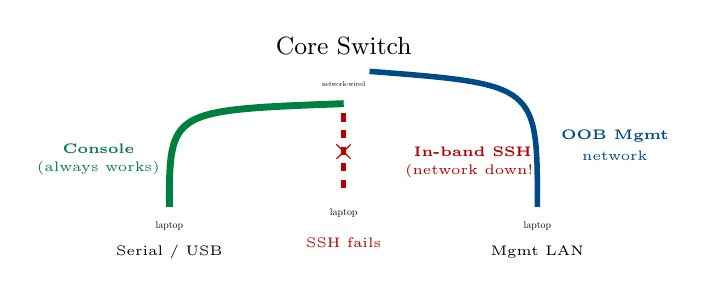
\begin{tikzpicture}[scale=0.82]
                    % Core switch
                    \node[switch] (sw) at (3.5,3.2) {\iconswitch[0.55cm]};
                    \node[font=\small] at (3.5,3.8) {Core Switch};
                    % In-band path (broken)
                    \draw[alertred, line width=2pt, dashed] (3.5,2.75) -- (3.5,1.6);
                    \node[font=\large, alertred] at (3.5,2.15) {\texttimes};
                    \node[font=\tiny\bfseries, alertred] at (5.5,2.15) {In-band SSH};
                    \node[font=\tiny, alertred] at (5.5,1.85) {(network down!)};
                    \node[laptop] at (3.5,1.2) {\iconlaptop[0.35cm]};
                    \node[font=\tiny, alertred] at (3.5,0.75) {SSH fails};
                    % Console path
                    \draw[networkgreen, line width=2.5pt]
                        (3.5,2.9) .. controls (0.8,2.8) .. (0.8,1.3);
                    \node[font=\tiny\bfseries, networkgreen] at (-0.3,2.2) {Console};
                    \node[font=\tiny, networkgreen] at (-0.3,1.9) {(always works)};
                    \node[laptop] at (0.8,1.0) {\iconlaptop[0.35cm]};
                    \node[font=\tiny] at (0.8,0.6) {Serial / USB};
                    % OOB path
                    \draw[rctcblue, line width=2pt]
                        (3.9,3.4) .. controls (6.5,3.2) .. (6.5,1.3);
                    \node[font=\tiny\bfseries, rctcblue] at (7.7,2.4) {OOB Mgmt};
                    \node[font=\tiny, rctcblue] at (7.7,2.1) {network};
                    \node[laptop] at (6.5,1.0) {\iconlaptop[0.35cm]};
                    \node[font=\tiny] at (6.5,0.6) {Mgmt LAN};
                \end{tikzpicture}
                \par\tiny\textit{When the production network is down, the console port (direct physical connection) and OOB management network provide alternative access paths to the device.}
            \end{center}
            \begin{alertblock}{\footnotesize Sysadmin Saying}
                \footnotesize ``When everything is on fire and SSH won't connect, the console port is your parachute.''
            \end{alertblock}
        \end{column}
    \end{columns}
\end{frame}

\articleonly{
\par\small\emph{A core switch is shown at the top center. Three paths lead from it: (1) A dashed red in-band SSH path goes downward to a laptop, but a red X and label "network down!" show it is broken. (2) A green console path curves left to another laptop labeled "Serial/USB," indicating the physical console port bypasses the network. (3) A blue OOB management path curves right to a third laptop labeled "Mgmt LAN," representing the separate out-of-band management network. The diagram illustrates fallback access methods when the primary network is unavailable.}\par
}

% =============================================================================
% SLIDE 29: Jump Boxes and APIs
% =============================================================================
\begin{frame}[t]{Jump Boxes and API-Based Management}
    \begin{columns}[T]
        \begin{column}{0.48\textwidth}
            \begin{block}{Jump Box (Bastion Host)}
                \begin{itemize}
                    \footnotesize
                    \item A \keyterm{jump box} is a \textbf{hardened, monitored server} at the boundary between external access and the secure internal network.
                    \item Admins first SSH or RDP \textit{to the jump box}, then connect from there to internal devices.
                    \item Benefits:
                        \begin{itemize}
                            \tiny
                            \item Single, audited entry point into the network.
                            \item Internal devices are never directly exposed externally.
                            \item All administrative sessions are logged for review.
                        \end{itemize}
                    \item This is an example of \keyterm{defense in depth}: even if an admin's laptop is compromised, the attacker cannot directly reach internal systems.
                \end{itemize}
            \end{block}
        \end{column}
        \begin{column}{0.49\textwidth}
            \begin{block}{API-Based Management}
                \begin{itemize}
                    \footnotesize
                    \item Modern network devices expose \keyterm{APIs} for \textbf{programmatic, automated} management.
                    \item \keyterm{REST API}: uses standard HTTP verbs (GET, POST, PUT, DELETE) and returns data in JSON. Most common.
                    \item \keyterm{NETCONF}: XML-based protocol over SSH, purpose-built for network configuration. Uses YANG data models.
                    \item \keyterm{gRPC / gNMI}: streaming telemetry used in modern SDN environments.
                \end{itemize}
            \end{block}
            \vspace{0.2em}
            \begin{exampleblock}{\footnotesize Why APIs Matter}
                \footnotesize Instead of manually SSH-ing into 200 switches one at a time, a single Python script calls each device's REST API and saves all configurations automatically --- in minutes, not hours.
            \end{exampleblock}
        \end{column}
    \end{columns}
\end{frame}

% =============================================================================
% SLIDE 30: Case Study 3
% =============================================================================
\begin{frame}[t]{Case Study: Dr.\ Eggman's Remote Management Crisis}
    \begin{casestudy}{Dr.\ Eggman's Remote Management Crisis}
        \footnotesize
        Dr.\ Eggman (Ivo Robotnik) manages robotics factories from his Egg Mobile command center.
        Assistant Orbot reports four urgent issues that need solving right now:

        \vspace{0.3em}
        \begin{center}
            \begin{tabular}{l p{8.0cm}}
                \toprule
                \textbf{Problem} & \textbf{Details} \\
                \midrule
                1 & Eggmanland factory switches are unresponsive over SSH. The entire production network is down. \\
                2 & The Death Egg's Windows management server needs a GUI session to install a critical patch. \\
                3 & Eggman wants to automate daily configuration backups from 200+ devices without manual logins. \\
                4 & A contractor (untrusted) needs one-time access to a single internal web portal. No software installation allowed. \\
                \bottomrule
            \end{tabular}
        \end{center}
    \end{casestudy}
    \begin{block}{Review Questions}
        \begin{enumerate}
            \footnotesize
            \item How does Eggman access the factory switches if the network is down?
            \item Which protocol should he use for the Windows server, and what mistake must he avoid?
            \item What management approach enables automated backup of 200 devices?
            \item What remote access type is correct for the untrusted contractor?
        \end{enumerate}
    \end{block}
\end{frame}

% =============================================================================
% SLIDE 31: Case Study 3 Solution
% =============================================================================
\begin{frame}[t]{Case Study Solution: Dr.\ Eggman's Remote Management}
    \begin{casesolution}{Dr.\ Eggman's Remote Management Crisis}
        \begin{enumerate}
            \footnotesize
            \item \textbf{Console port or out-of-band (OOB) management.} SSH is an in-band tool that requires a working network. When the production network is down, Eggman must use a physical console cable directly connected to each switch, or a dedicated OOB management network that is independent of the production data plane.
            \item \textbf{RDP (TCP 3389)} for the Windows GUI session. The critical mistake to avoid: \textit{never expose port 3389 directly to the internet}. Eggman should connect via VPN first, then RDP to the server on the internal network --- or route through a jump box for additional audit logging.
            \item \textbf{REST API or NETCONF.} A script can call each device's API endpoint sequentially or in parallel, retrieving and saving configurations automatically. Manual SSH logins to 200 devices would take hours and introduce human error.
            \item \textbf{Clientless SSL VPN.} Browser-based, no installation required, and access can be scoped to \textit{only} that one web portal. This limits the blast radius if the contractor's device is compromised.
        \end{enumerate}
    \end{casesolution}
    \begin{alertblock}{\footnotesize Real-World Reminder}
        \footnotesize These map to real incidents: exposed RDP leads to ransomware; no OOB means a misconfiguration bricks a remote site for days; manual config management on 200 devices creates drift and errors. Plan for failure \textit{before} it happens.
    \end{alertblock}
\end{frame}

% =============================================================================
% SLIDE 32: Module Summary
% =============================================================================
\section*{Module Summary}

\begin{frame}[t,allowframebreaks]{Module 13 Summary}
    \small
    \textbf{WAN and Internet Connectivity:}
    \begin{itemize}
        \item A \keyterm{WAN} connects geographically separated networks over provider-owned infrastructure (Layers 1--3).
        \item \keyterm{DSL}: dedicated copper phone line; speed degrades with distance. \keyterm{Cable (DOCSIS)}: shared coaxial cable; faster but contended at neighborhood node.
        \item \keyterm{FTTC}: fiber runs to a street cabinet; copper covers the last 100--300 m. \keyterm{FTTP/FTTH}: pure fiber to the premises via an ONT; best speed and latency.
        \item \keyterm{Cellular WAN} (4G/5G): mobile broadband; used for primary or failover WAN. \keyterm{Satellite}: GEO = high latency ($\sim$600 ms); LEO = lower latency ($\sim$40 ms).
    \end{itemize}
    \framebreak
    \textbf{Virtual Private Networks:}
    \begin{itemize}
        \item A \keyterm{VPN} = tunneling + encryption + authentication over an untrusted network.
        \item \keyterm{Tunneling / encapsulation}: private packet is wrapped inside a public-addressed outer packet; decapsulated at the far endpoint.
        \item Protocols: PPTP (broken, avoid); L2TP/IPsec; OpenVPN; WireGuard; SSTP.
        \item \keyterm{IPsec}: \textbf{AH} (auth/integrity, no encryption) vs.\ \textbf{ESP} (auth/integrity + encryption --- use this). \textbf{Transport mode} (host-to-host); \textbf{Tunnel mode} (gateway VPNs).
        \item \keyterm{IKE}: Phase 1 authenticates peers and builds a secure channel; Phase 2 negotiates session keys inside that channel.
        \item \keyterm{Client-to-site}: individual user + VPN client software; full or split tunnel option.
        \item \keyterm{Clientless SSL VPN}: browser only; web resources only; no software needed.
        \item \keyterm{Site-to-site}: two routers/firewalls form a permanent tunnel; transparent to end users.
    \end{itemize}
    \framebreak
    \textbf{Remote Management:}
    \begin{itemize}
        \item \keyterm{SSH} (TCP 22): encrypted CLI; key-based auth preferred; always use version 2.
        \item \keyterm{Telnet} (TCP 23): plaintext --- disable everywhere; replace with SSH.
        \item \keyterm{RDP} (TCP 3389): encrypted GUI for Windows; never expose directly to the internet --- use VPN or a jump box.
        \item \keyterm{Console port}: physical serial/USB connection; bypasses the network entirely; last resort when network access is down.
        \item \keyterm{Out-of-band (OOB) management}: dedicated management network independent of the production network; survives production outages.
        \item \keyterm{Jump box (bastion host)}: hardened pivot point; admins connect here first, then to internal devices; enables audit logging and limits internal exposure.
        \item \keyterm{REST API} / \keyterm{NETCONF} / gRPC: programmatic management for automation at scale; REST returns JSON over HTTPS; NETCONF uses XML/YANG over SSH.
    \end{itemize}
\end{frame}

\end{document}
